\section{Introduction}\label{sec:intro}

A central goal of machine learning research is to develop universal architectures capable of learning and reasoning across a wide range of tasks and data modalities. A compelling hypothesis is that human and animal intelligence can be explained by a small set of fundamental principles~\citep{marcus2003algebraic}. There is, however, a tension between the goal of creating a general architecture and the need to incorporate inductive biases that are beneficial for specific tasks~\citep{wolpert1995no,baxter2000model}. When faced with finite training data and numerous solutions to empirical risk minimization, inductive biases steer the learning algorithm towards solutions with desirable properties, enhancing data efficiency and generalization.
% To-Add: Different neural architectures have different sets of inductive biases, designed for specific tasks~\citep{goyal2022inductive,battaglia,geometricdeeplearningpaper}.?
In machine intelligence, the scientific challenge is to identify a complete set of fundamental inductive biases with broad applicability to real-world problems that enable robust, flexible, and data-efficient learning.

The Transformer architecture~\citep{vaswani2017attention} offers a promising candidate for the foundations of a versatile, general-purpose machine learning framework. By operating over sets or sequences of objects, Transformers are able to support highly-general input and output modalities. More importantly, neural attention provides an effective computational mechanism for routing sensory information between different elements in the input, enabling iterative contextual processing. This has led to remarkable empirical success across several domains, including language~\citep{radfordImprovingLanguageUnderstanding2018,devlinBERTPretrainingDeep2019,radford2019language,kaplan2020scalinglawsneurallanguage,brown2020languagemodelsfewshotlearners} and visual processing~\citep{dosovitskiyImageWorth16x162020,carion2020end,zhai2022scaling}.
\aanote{add several more citations for each?}

% Different neural architectures have different sets of inductive biases. The transformer architecture provides a promising foundation for a general-purpose machine learning framework owing to its attention mechanism
 
\aanote{trim this paragraph slightly to save a line}
However, recent work on relational learning has shown that Transformers struggle to efficiently learn tasks involving relational reasoning~\citep{lake2018generalization,barrett2018measuring,santoroSimpleNeuralNetwork2017,santoroRelationalRecurrentNeural2018,shanahanExplicitlyRelationalNeurala,webbEmergentSymbolsBinding2021,webbRelationalBottleneckInductive2024,kergNeuralArchitectureInductive2022,altabaa2024abstractors,altabaaLearningHierarchicalRelational2024}. Relational reasoning is a central component of generally intelligent systems, and is believed to underlie human abilities for abstraction and systematic generalization~\citep{snow1984topography,kemp2008discovery,holyoak2012analogy}. The power of relational reasoning lies in its capacity to generate inferences and generalizations in systematic and novel ways, which can ultimately lead to universal inductive generalization from a finite set of observations to an infinite set of novel instances~\citep{goyal2022inductive}. The lack of support for efficient and robust relational learning remains a major limitation of the Transformer framework.

In this work, drawing analogy to neural systems in the brain~\citep{newman1997neural}, we distinguish between two types of information: \textit{sensory} information which encodes the properties of individual objects, and \textit{relational} information which encodes the relationships between objects. Accordingly, we posit the following explanation for the Transformer's limited abilities in relational learning: while neural attention provides a powerful mechanism for routing \textit{sensory} information in the input, the Transformer lacks an explicit computational mechanism for routing and processing \textit{relational} information between objects in the input. We argue that a unified architecture for general machine intelligence requires computational mechanisms and inductive biases for processing both sensory and relational information. Towards this goal, we propose an extension of the Transformer framework which enables explicit routing and processing of both sensory and relational information.

To understand our proposed method at a high-level, it is useful to view standard Transformers as an instance of a broader neural message-passing computational paradigm that consists of iterative information retrieval followed by local processing. In the general form of a message-passing procedure, a set of objects $x_1,\ldots, x_n$ are processed via an iterative application of
\begin{equation}\label{eq:intro_message_passing}
  \begin{split}
    \text{(Information Retrieval)} \quad x_i &\gets \mathrm{Aggregate}\bigparen{x_i, \set{m_{j \to i}}_{j=1}^{n}}, \\
    \text{(Local Processing)} \quad x_i &\gets \mathrm{Process}(x_i).
  \end{split}
\end{equation}
In Transformers, the information retrieval step corresponds to the self-attention mechanism, where the message sent from object $j$ to object $i$ is an encoding of the sender's \textit{sensory} features, $m_{j \to i} = \phi_v(x_j)$. These messages are then aggregated according to some selection criterion based on the receiver's features, determined by softmax attention scores.

To enable explicit relational representation learning, we propose a novel attention mechanism, dubbed \textit{relational attention}, that selectively attends to and routes relational information between objects. In relational attention, the message from the sender object to the receiver object consists of a set of relations between them, which can be expressed as $m_{j \to i} = r(x_i, x_j)$. Here, the relation $r(\cdot, \cdot)$ models a series of comparisons between the pair of objects across different feature dimensions using inner products of feature maps. We integrate this with the standard attention mechanism of Transformers, yielding a variant of multi-head attention for processing both sensory and relational information in parallel. This \textit{Dual Attention} architecture disentangles these two types of information during the aggregation phase, while integrating them in the information processing stage.

The contributions of this paper are summarized as follows:

\begin{itemize}[left=5pt]
  \item \textit{\textbf{A neural mechanism for routing and processing relational information.}} We introduce a new \textit{relational attention} mechanism that disentangles relational information from sensory information. While standard self-attention models the retrieval of sensory information, relational attention models the retrieval of relational information.
  \item \textit{\textbf{An architectural extension of the Transformer for joint sensory-relational processing.}} We introduce an extension of the Transformer architecture that integrates sensory and relational information through \textit{Dual Attention}---a form of multi-head attention with two distinct types of attention heads. Standard self-attention heads encode sensory information, while relational attention heads encode relational information.
  \item \textit{\textbf{Empirically evaluating the promise of relational computational mechanisms.}} While relational reasoning is believed to be an essential component of general intelligence, the success of relational inductive biases in machine learning has so far been mainly limited to synthetic tasks, despite recent advances in relational architectures~\citep{santoroSimpleNeuralNetwork2017,santoroRelationalRecurrentNeural2018,shanahanExplicitlyRelationalNeurala,webbEmergentSymbolsBinding2021,webbRelationalBottleneckInductive2024,kergNeuralArchitectureInductive2022,altabaa2024abstractors,altabaaLearningHierarchicalRelational2024}. We evaluate the \textit{Dual Attention Transformer} architecture on a diverse set of tasks ranging from synthetic relational benchmarks to complex real-world tasks such as language modeling and visual processing. Our results demonstrate that incorporating explicit relational computational mechanisms into the Transformer architecture leads to significant performance gains in terms of data efficiency and parameter efficiency.
\end{itemize}

\begin{figure}[t]
  \centering
  \begin{subfigure}[t]{0.415384615\textwidth} % 0.9 * 3 / 6.5
    \centering
    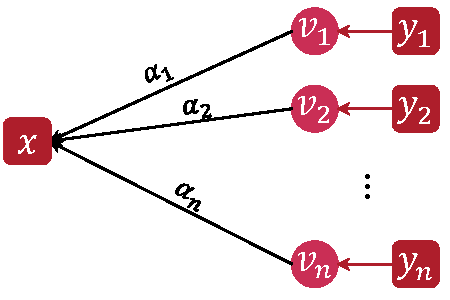
\includegraphics[width=\textwidth]{figs/sensory_retrieval.pdf} % size: 3 x 2 in
    \caption{$\Attn(x, \ys)$}%: Retrieval of sensory information by standard attention.}
  \end{subfigure}
  \qquad
  \begin{subfigure}[t]{0.484615385\textwidth} % 0.9 * 3.5 / 6.5
    \centering
    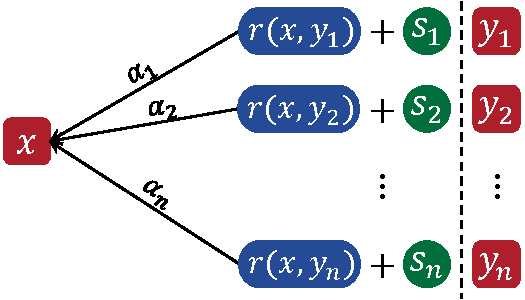
\includegraphics[width=\textwidth]{figs/relational_retrieval.pdf} % size 3.5 x 2 in
    \caption{$\RelAttn(x, \ys)$}%: Retrieval of relational information by relational attention.}
  \end{subfigure}
  % 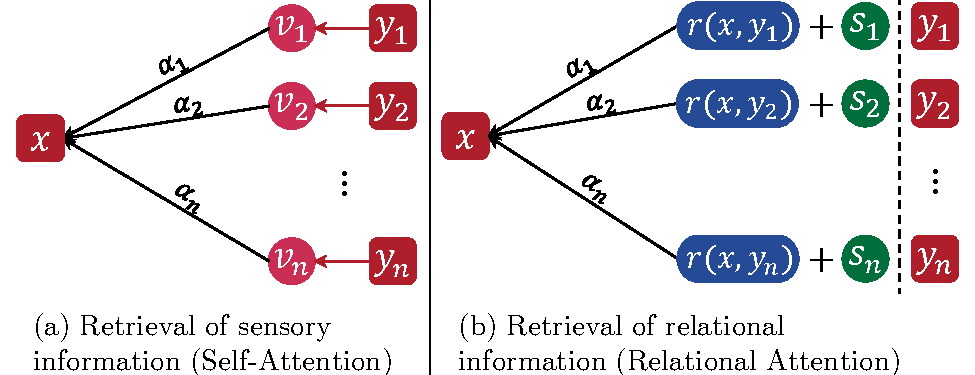
\includegraphics[width=0.8\textwidth]{figs/attn_fig_combined_noqeuerykey.pdf}
  \caption{Standard self-attention retrieves sensory information $v_i$ about the attributes of individual objects while \textit{relational attention} retrieves relational information $r(x, y_i)$ about the relationship between the objects in the context and the receiver.
  Each relation is tagged with a symbol $s_i$ which acts as an abstract variable identifying the sender.
  In both cases, information is aggregated according to the attention scores $\alpha_i$, which are computed by a softmax over inner products of queries and keys.
  }\label{fig:selfattn_relattn}
  \vskip-7pt
\end{figure}

% \todo{Add short related work section? --- emphasize that previous work on relational learning has been limited to synthetic settings and has yet to demonstrate the general applicability of relational computational mechanisms to complex real-world tasks. ``With minor caveats, these architectures are narrow in domain and have primarily been applied to synthetic settings. By contrast, our goal/target in this paper is to study the effects/potential beneifts of relational inductive biases and computational mechanisms as a component of general machine intelligence frameworks in complex real-world domains''}